\documentclass[a4paper, 14pt]{extarticle}

% Поля
%--------------------------------------
\usepackage{geometry}
\geometry{a4paper,tmargin=2cm,bmargin=2cm,lmargin=3cm,rmargin=1cm}
%--------------------------------------


%Russian-specific packages
%--------------------------------------
\usepackage[T2A]{fontenc}
\usepackage[utf8]{inputenc} 
\usepackage[english, main=russian]{babel}
%--------------------------------------

\usepackage{textcomp}

% Красная строка
%--------------------------------------
\usepackage{indentfirst}               
%--------------------------------------             


%Graphics
%--------------------------------------
\usepackage{graphicx}
\graphicspath{ {./images/} }
\usepackage{wrapfig}
%--------------------------------------

% Полуторный интервал
%--------------------------------------
\linespread{1.3}                    
%--------------------------------------

%Выравнивание и переносы
%--------------------------------------
% Избавляемся от переполнений
\sloppy
% Запрещаем разрыв страницы после первой строки абзаца
\clubpenalty=10000
% Запрещаем разрыв страницы после последней строки абзаца
\widowpenalty=10000
%--------------------------------------

%Списки
\usepackage{enumitem}

%Подписи
\usepackage{caption} 

%Гиперссылки
\usepackage{hyperref}

\hypersetup {
	unicode=true
}

%Рисунки
%--------------------------------------
\DeclareCaptionLabelSeparator*{emdash}{~--- }
\captionsetup[figure]{labelsep=emdash,font=onehalfspacing,position=bottom}
%--------------------------------------

\usepackage{tempora}

%Листинги
%--------------------------------------
\usepackage{listings}
\lstset{
  basicstyle=\ttfamily\footnotesize, 
  %basicstyle=\footnotesize\AnkaCoder,        % the size of the fonts that are used for the code
  breakatwhitespace=false,         % sets if automatic breaks shoulbd only happen at whitespace
  breaklines=true,                 % sets automatic line breaking
  captionpos=t,                    % sets the caption-position to bottom
  inputencoding=utf8,
  frame=single,                    % adds a frame around the code
  keepspaces=true,                 % keeps spaces in text, useful for keeping indentation of code (possibly needs columns=flexible)
  keywordstyle=\bf,       % keyword style
  numbers=left,                    % where to put the line-numbers; possible values are (none, left, right)
  numbersep=5pt,                   % how far the line-numbers are from the code
  xleftmargin=25pt,
  xrightmargin=25pt,
  showspaces=false,                % show spaces everywhere adding particular underscores; it overrides 'showstringspaces'
  showstringspaces=false,          % underline spaces within strings only
  showtabs=false,                  % show tabs within strings adding particular underscores
  stepnumber=1,                    % the step between two line-numbers. If it's 1, each line will be numbered
  tabsize=2,                       % sets default tabsize to 8 spaces
  title=\lstname                   % show the filename of files included with \lstinputlisting; also try caption instead of title
}
%--------------------------------------

%%% Математические пакеты %%%
%--------------------------------------
\usepackage{amsthm,amsfonts,amsmath,amssymb,amscd}  % Математические дополнения от AMS
\usepackage{mathtools}                              % Добавляет окружение multlined
\usepackage[perpage]{footmisc}
%--------------------------------------

%--------------------------------------
%			НАЧАЛО ДОКУМЕНТА
%--------------------------------------

\begin{document}

%--------------------------------------
%			ТИТУЛЬНЫЙ ЛИСТ
%--------------------------------------
\begin{titlepage}
\thispagestyle{empty}
\newpage


%Шапка титульного листа
%--------------------------------------
\vspace*{-60pt}
\hspace{-65pt}
\begin{minipage}{0.3\textwidth}
\hspace*{-20pt}\centering

\includegraphics[width=\textwidth]{emblem}
\end{minipage}
\begin{minipage}{0.67\textwidth}\small \textbf{
\vspace*{-0.7ex}
\hspace*{-6pt}\centerline{Министерство науки и высшего образования Российской Федерации}
\vspace*{-0.7ex}
\centerline{Федеральное государственное бюджетное образовательное учреждение }
\vspace*{-0.7ex}
\centerline{высшего образования}
\vspace*{-0.7ex}
\centerline{<<Московский государственный технический университет}
\vspace*{-0.7ex}
\centerline{имени Н.Э. Баумана}
\vspace*{-0.7ex}
\centerline{(национальный исследовательский университет)>>}
\vspace*{-0.7ex}
\centerline{(МГТУ им. Н.Э. Баумана)}}
\end{minipage}
%--------------------------------------

%Полосы
%--------------------------------------
\vspace{-25pt}
\hspace{-35pt}\rule{\textwidth}{2.3pt}

\vspace*{-20.3pt}
\hspace{-35pt}\rule{\textwidth}{0.4pt}
%--------------------------------------

\vspace{1.5ex}
\hspace{-35pt} \noindent \small ФАКУЛЬТЕТ\hspace{80pt} <<Информатика и системы управления>>

\vspace*{-16pt}
\hspace{47pt}\rule{0.83\textwidth}{0.4pt}

\vspace{0.5ex}
\hspace{-35pt} \noindent \small КАФЕДРА\hspace{50pt} <<Теоретическая информатика и компьютерные технологии>>

\vspace*{-16pt}
\hspace{30pt}\rule{0.866\textwidth}{0.4pt}
  
\vspace{11em}

\begin{center}
\Large {\bf Лабораторная работа № 5} \\ 
\large {\bf по курсу <<Языки и методы программирования>>} \\
\large <<Монады в языке Java>> 
\end{center}\normalsize

\vspace{8em}


\begin{flushright}
  {Студент группы ИУ9-21Б Горбунов А. Д. \hspace*{15pt}\\ 
  \vspace{2ex}
  Преподаватель Посевин Д. П.\hspace*{15pt}}
\end{flushright}

\bigskip

\vfill
 

\begin{center}
\textsl{Москва 2023}
\end{center}
\end{titlepage}
%--------------------------------------
%		КОНЕЦ ТИТУЛЬНОГО ЛИСТА
%--------------------------------------

\renewcommand{\ttdefault}{pcr}

\setlength{\tabcolsep}{3pt}
\newpage
\setcounter{page}{2}

\section{Задание}\label{Sect::task}
Множество строк вида «Фамилия Имя Отчество, год рождения» с операциями:

1. порождение потока имён;

2. поиск в множестве самого старшего обладателя указанной фамилии.

Проверить работу первой операции нужно путём поиска наиболее часто встречающегося имени.
\section{Результаты}\label{Sect::res}

Исходный код программы представлен в листинге~\ref{lst:code1}, ~\ref{lst:code2}, ~\ref{lst:code3}, ~\ref{lst:code4}, ~\ref{lst:code5}

\begin{figure}[!htb]
\begin{lstlisting}[language={},caption={класс Test},label={lst:code1}]
public class Test {
    public static void main(String[] args) {
        PersonTable t = new PersonTable();
        t.add("a", "aa", "aaa", 1);
        t.add("b", "bb", "bbb", 10);
        t.add("c", "asf", "ccc", 3);
        t.add("d", "dd", "ddd", 4);
        t.add("gc", "rf", "sv", 5);
        t.add("gac", "cc", "fr", 2);
        t.add("gac", "cc", "fr", 7);
        t.add(new Person("as","cc","kef", 8));
        t.firstNameStream().forEach(x-> System.out.println(x.getKey()));
        System.out.println(t.getMaxAge("gac").get().age);
    }
}
\end{lstlisting}
\end{figure}

\begin{figure}[!htb]
\begin{lstlisting}[language={},caption={класс PersonTable},label={lst:code2}]
import java.util.ArrayList;
import java.util.HashMap;
import java.util.Map;
import java.util.Optional;
import java.util.stream.Stream;
public class PersonTable {
    HashMap<String, Person> Table;
    HashMap<String, Integer> firstnames;
\end{lstlisting}
\end{figure}

\begin{figure}[!htb]
\begin{lstlisting}[language={},caption={класс PersonTable(продолжение)},label={lst:code3}]
    private int maxAge = -1;
    private int maxNumbersFirstname = 1;
    PersonTable() {
        Table = new HashMap<>();
        firstnames = new HashMap<>();
    }
    void add(Person p) {
        if(firstnames.containsKey(p.firstname)){
            Integer f = firstnames.get(p.firstname);
            firstnames.remove(p.firstname);
            firstnames.put(p.firstname, f+1);
            if(maxNumbersFirstname <f+1){
                maxNumbersFirstname = f+1;
            }

        }else{
            firstnames.put(p.firstname, 1);
        }
        Table.put(new String[]{p.firstname, p.lastname,p.surname}, p);

        if(maxAge< p.age){
            maxAge=p.age;
        }
    }
    void add(String lastname, String firstname, String surname, int age) {

        if(firstnames.containsKey(firstname)){
            Integer f = firstnames.get(firstname);
            firstnames.remove(firstname);
            firstnames.put(firstname, f+1);
            if(maxNumbersFirstname <f+1){maxNumbersFirstname = f+1;}
        }else{firstnames.put(firstname, 1); }
        Table.put(new String[]{firstname, lastname, surname}, new Person(lastname, firstname, surname, age));
        if(maxAge< age){maxAge= age;}
    }
    public Stream<Map.Entry<String, Integer>> firstNameStream() {
        ArrayList<Map.Entry<String, Integer>> result = new ArrayList<>();
        firstnames.entrySet().stream().filter(x-> firstnames.get(x.getKey()) == getMaxNumbersFirstname()).forEach(x -> result.add(x));
        return result.stream();
    }
    public Optional<Person> getMaxAge(String lastname) {
        Optional<Person> result = Optional.empty();
        Optional<Map.Entry<String[], Person>> tmp = Table.entrySet().stream().sorted(new NameComparator()).filter(x-> (x.getKey()[1].equals(lastname))).findFirst();
        if (tmp.isPresent()) {
            result = Optional.ofNullable(tmp.get().getValue());}
        return result;
    }
    public int getMaxNumbersFirstname(){
        return maxNumbersFirstname;}
}
\end{lstlisting}
\end{figure}

\begin{figure}[!htb]
\begin{lstlisting}[language={},caption={класс Person},label={lst:code4}]
public class Person {
    int age;
    String firstname, lastname, surname;
    public Person (String lastname, String firstname, String surname, int age) {
        this.lastname = lastname;
        this.firstname = firstname;
        this.surname = surname;
        this.age = age;
    }
}
\end{lstlisting}
\end{figure}

\begin{figure}[!htb]
\begin{lstlisting}[language={},caption={класс NameComparator},label={lst:code5}]
import java.util.*;
class NameComparator implements Comparator<Map.Entry<String[], Person>> {
    public int compare(Map.Entry<String[], Person>  a, Map.Entry<String[], Person> b) {
        int a0, b0;
        a0 = a.getValue().age;
        b0 = b.getValue().age;
        if (a0 < b0) { return 1; }
        if (a0 == b0) { return 0; }
        return -1;
    }
}
\end{lstlisting}
\end{figure}

\begin{figure}[!htb]
Результат запуска представлен на рисунке ~\ref{fig:picture_1.png}, ~\ref{fig:picture_2.png}, ~\ref{fig:picture_3.png}.
\end{figure}

\begin{figure}[!htb]
	\centering
	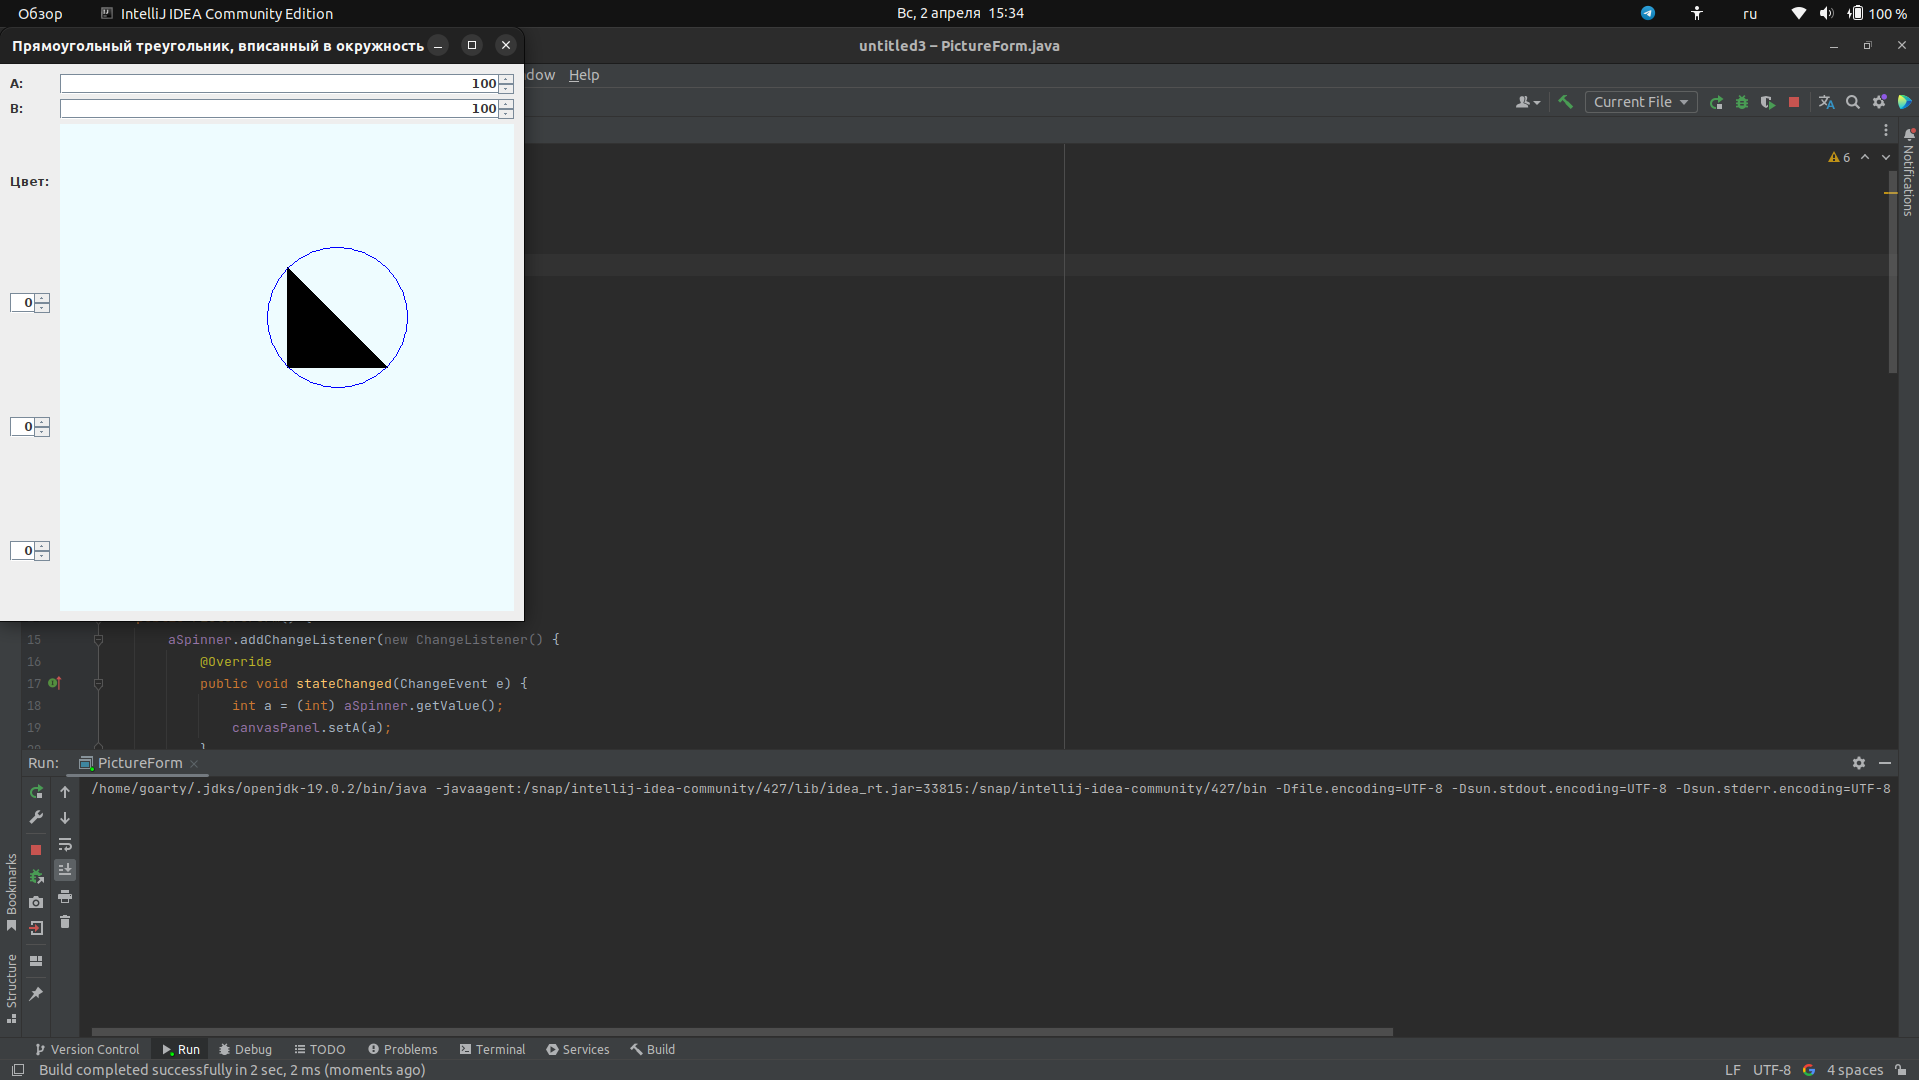
\includegraphics[width=0.8\textwidth]{picture_1.png}
\caption{Вывод программы(3 три повторяющихся имени cc и две повторяющиеся фамилии gac(age 7 и 2))}
\label{fig:picture_1.png}
\end{figure}

\begin{figure}[!htb]
	\centering
	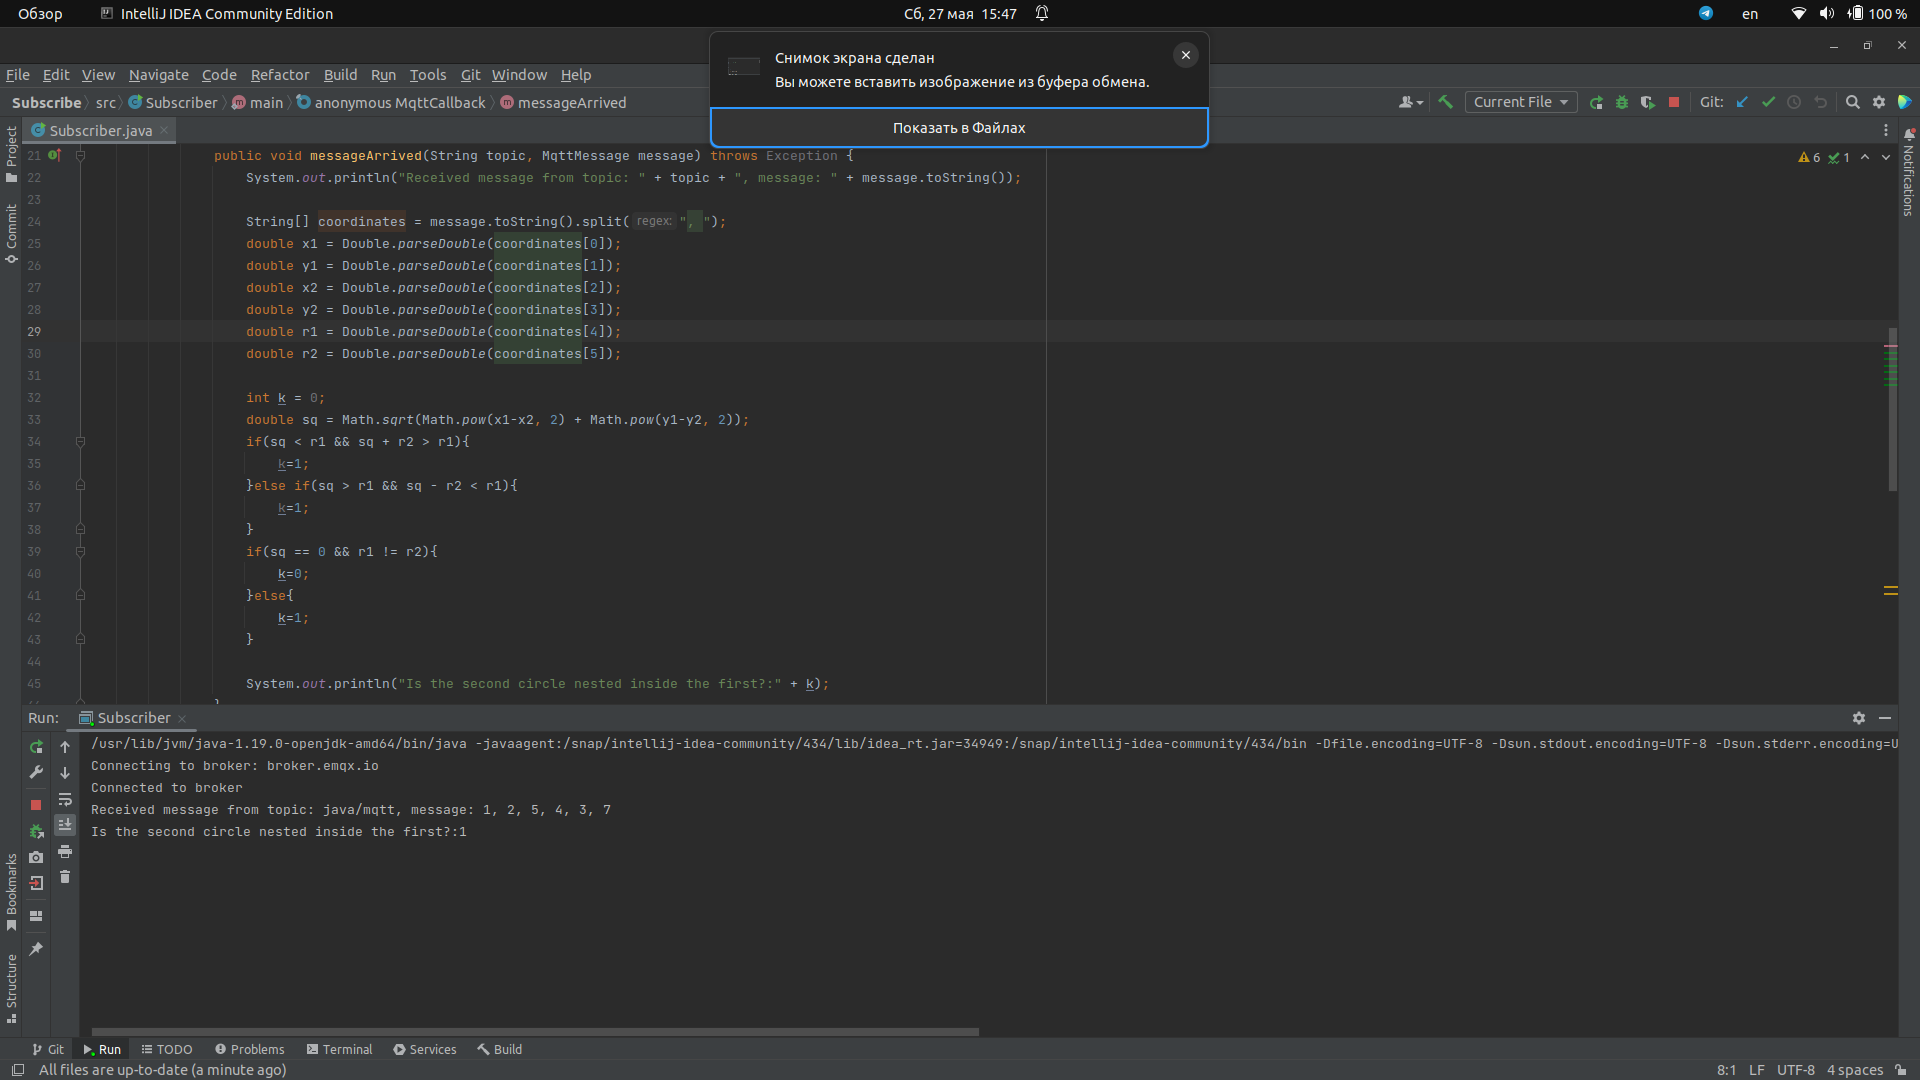
\includegraphics[width=0.8\textwidth]{picture_2.png}
\caption{Вывод программы(нет одинаковых имён и только одна фамилия gas (age 7))}
\label{fig:picture_2.png}
\end{figure}

\begin{figure}[!htb]
	\centering
	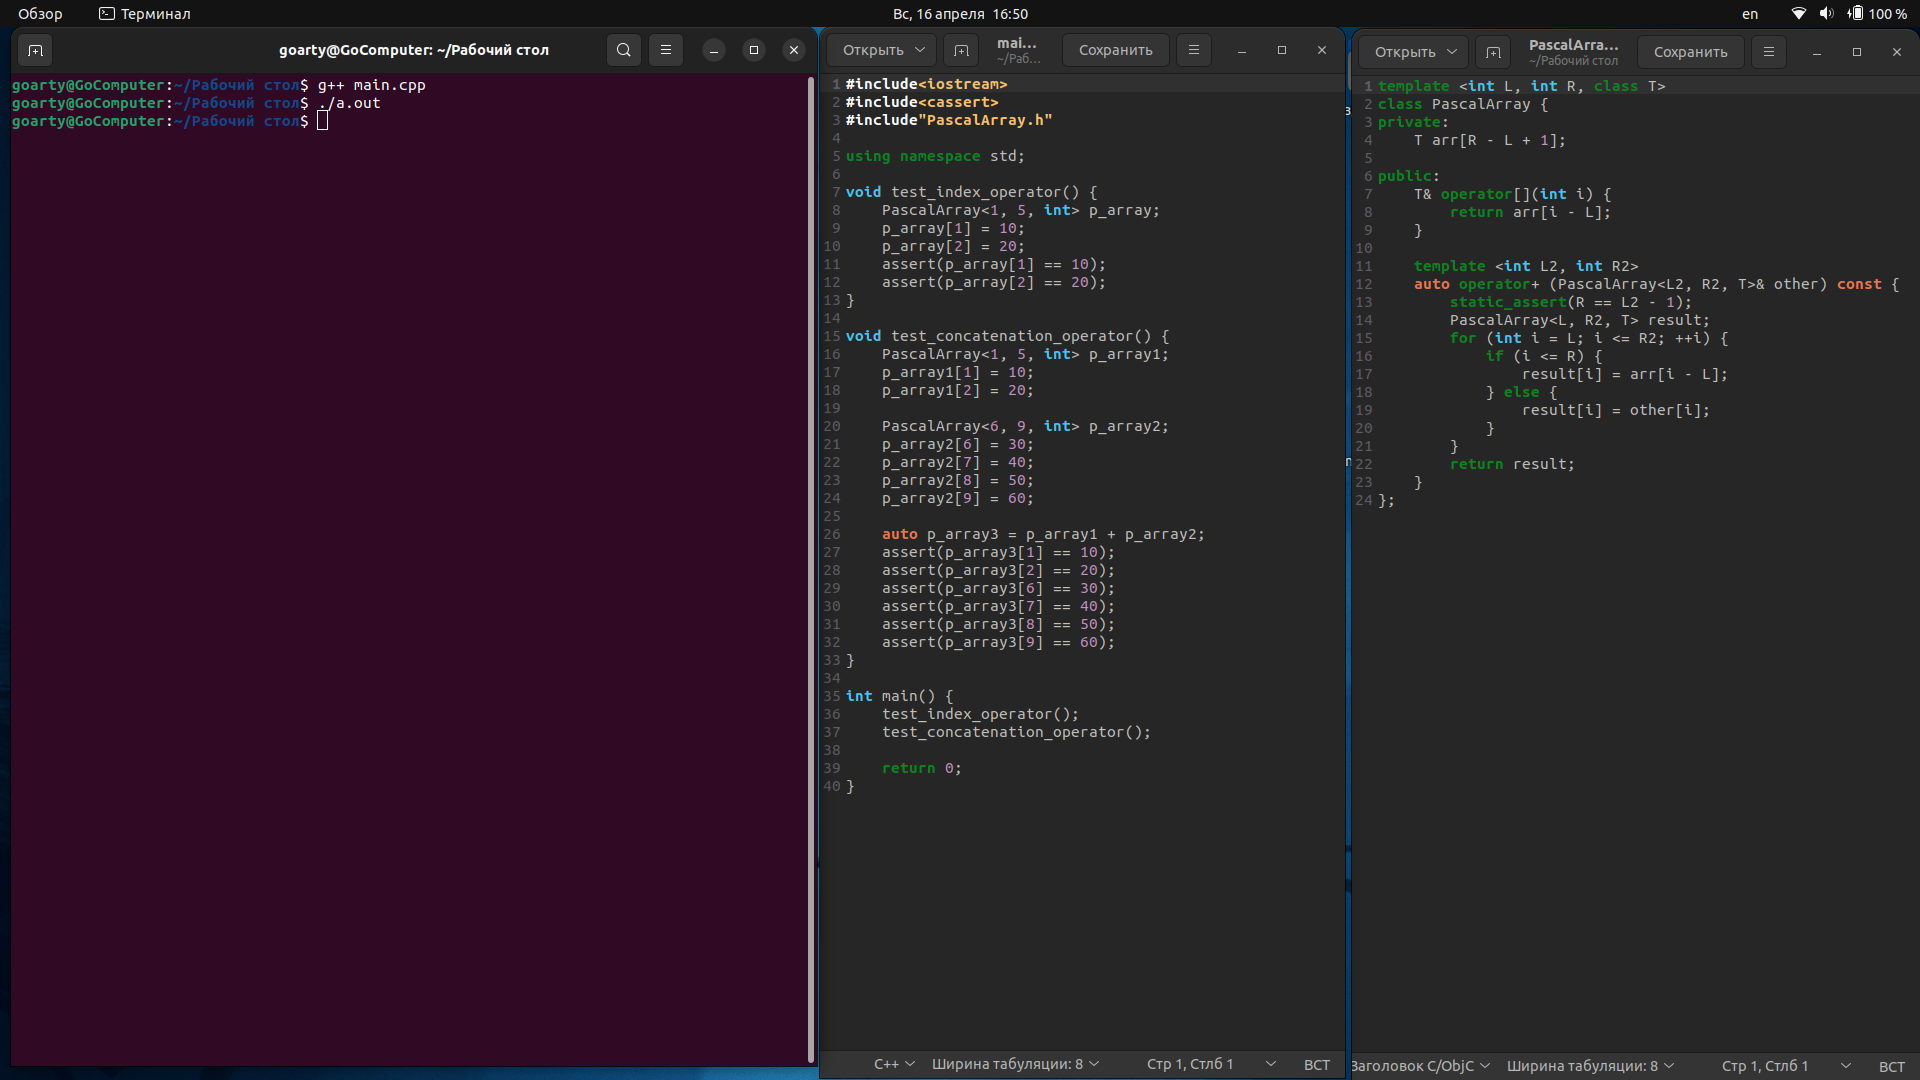
\includegraphics[width=0.8\textwidth]{picture_3.png}
\caption{Вывод программы(всех зовут cc и у всех фамилия gas)}
\label{fig:picture_3.png}
\end{figure}

\end{document}

